\section{RandN Class Reference}
\label{classRandN}\index{RandN@{RandN}}
Inheritance diagram for RandN::\begin{figure}[H]
\begin{center}
\leavevmode
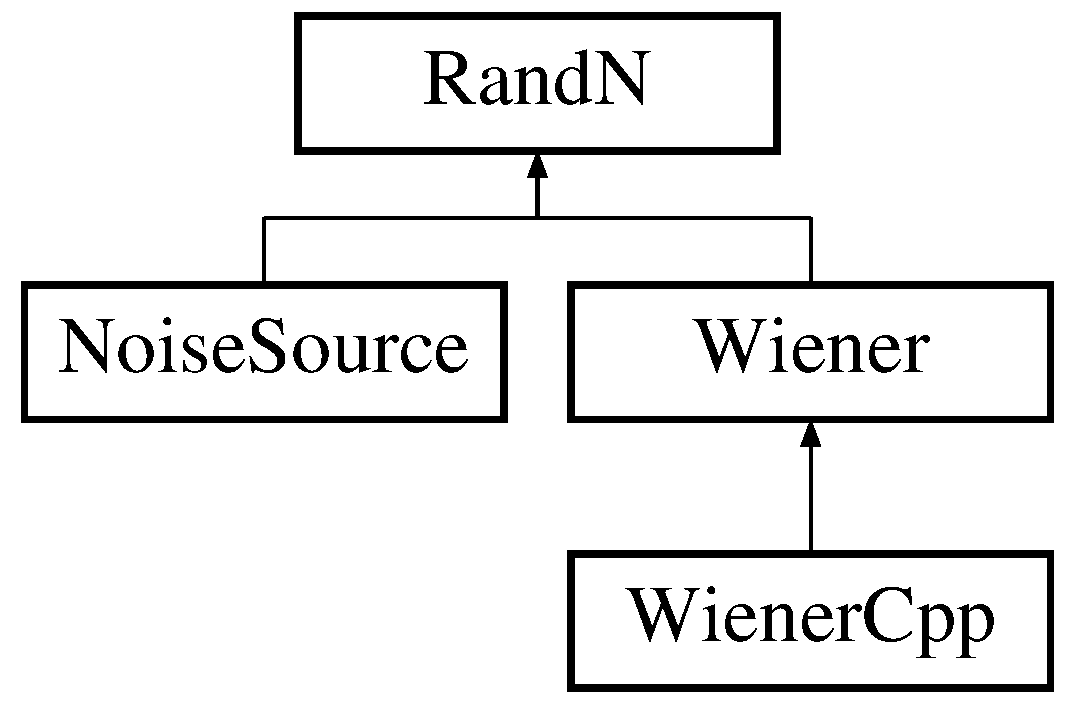
\includegraphics[height=3cm]{classRandN}
\end{center}
\end{figure}


\subsection{Detailed Description}
An object which uses the randn function. 

This class implements a random variable with normal distribution (gaussian). \subsection*{Public Member Functions}
\begin{CompactItemize}
\item 
{\bf RandN} ()\label{classRandN_e842af49a10a6dc84bdcf2a0cc643f98}

\begin{CompactList}\small\item\em Construct. \item\end{CompactList}\item 
{\bf $\sim$RandN} ()\label{classRandN_ffb47d3d5cb0d2c28e4d7b84f5ee81ff}

\begin{CompactList}\small\item\em Destruct. \item\end{CompactList}\item 
double {\bf dRandN} ()
\begin{CompactList}\small\item\em Retrieve random variable. \item\end{CompactList}\end{CompactItemize}


\subsection{Member Function Documentation}
\index{RandN@{RandN}!dRandN@{dRandN}}
\index{dRandN@{dRandN}!RandN@{RandN}}
\subsubsection[dRandN]{\setlength{\rightskip}{0pt plus 5cm}double RandN::dRandN ()}\label{classRandN_0f821b3a122bbd285978503e504bd5f8}


Retrieve random variable. 

This function generates one random variable. The returend values are normally (Gaussian) distributed, with a mean of 0.0 and a variance of 1.0. The method used is the Polar-Masaglia method, which is the quickest known so far. 